% 2D Example Translation
%
% File:         2d-translation.tex
% Author:       Bob Walton (walton@acm.org)
% Date:      	Thu Dec 20 10:54:59 EST 2012
  
\documentclass{minimal}
\usepackage[paperheight=3in,paperwidth=2in,
            height=3in,hoffset=0.05in,
	    voffset=0.05in,left=0in,width=2in]{geometry}
\usepackage{color}
\usepackage[usenames]{xcolor}
\usepackage{tikz}
\usetikzlibrary{arrows}
\begin{document}
\raggedright
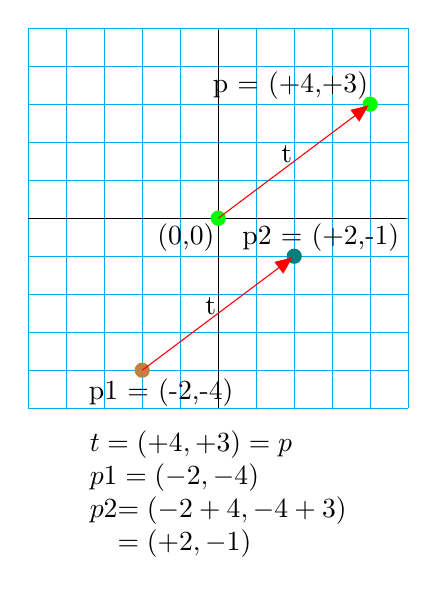
\begin{tikzpicture}[x=0.190in,y=0.190in]
\begin{scope}[yshift=1in,>=triangle 45,shorten >=0.01in]
    \draw[cyan] (-5,-5) grid[step=1] (5,5);
    \draw[black] (-5,0) -- (+5,0);
    \draw[black] (0,-5) -- (0,+5);
    \fill[green] (0,0) circle(0.2) + (-0.85,-0.5) node[black]{(0,0)};
    \fill[green] (+4,+3) circle(0.2) + (-2.1,+0.5) node[black]{p = (+4,+3)};
    \draw[red,->] (0,0) -- (+4,+3);
    \draw[black] (1.8,1.7) node{t};

    \fill[brown] (-2,-4) circle(0.2) + (+0.5,-0.6) node[black]{p1 = (-2,-4)};
    \fill[teal] (+2,-1) circle(0.2) + (+0.7,+0.5) node[black]{p2 = (+2,-1)};
    \draw[red,->] (-2,-4) -- (+2,-1);
    \draw[black] (-0.2,-2.3) node{t};
\end{scope}

\begin{scope}
\draw (0,-2) node {
    $\begin{array}{l}
    t = (+4,+3) = p \\
    p1 = (-2,-4) \\
    p2 \begin{array}[t]{@{}l@{}}
       = (-2+4,-4+3) \\
       = (+2,-1)
       \end{array}
    \end{array}$
    };
\end{scope}
\end{tikzpicture}
\end{document}
